%%%%%%%%%%%%  Generated using docx2latex.com  %%%%%%%%%%%%%%

%%%%%%%%%%%%  v2.0.0-beta  %%%%%%%%%%%%%%

\documentclass[12pt]{article}
\usepackage{amsmath}
\usepackage{latexsym}
\usepackage{amsfonts}
\usepackage[normalem]{ulem}
\usepackage{array}
\usepackage{amssymb}
\usepackage{graphicx}
\usepackage[backend=biber,
style=numeric,
sorting=none,
isbn=false,
doi=false,
url=false,
]{biblatex}\addbibresource{bibliography.bib}

\usepackage{subfig}
\usepackage{wrapfig}
\usepackage{wasysym}
\usepackage{enumitem}
\usepackage{adjustbox}
\usepackage{ragged2e}
\usepackage[svgnames,table]{xcolor}
\usepackage{tikz}
\usepackage{longtable}
\usepackage{changepage}
\usepackage{setspace}
\usepackage{hhline}
\usepackage{multicol}
\usepackage{tabto}
\usepackage{float}
\usepackage{multirow}
\usepackage{makecell}
\usepackage{fancyhdr}
\usepackage[toc,page]{appendix}
\usepackage[hidelinks]{hyperref}
\usetikzlibrary{shapes.symbols,shapes.geometric,shadows,arrows.meta}
\tikzset{>={Latex[width=1.5mm,length=2mm]}}
\usepackage{flowchart}\usepackage[paperheight=11.69in,paperwidth=8.27in,left=0.98in,right=0.98in,top=0.98in,bottom=0.98in,headheight=1in]{geometry}
\usepackage[utf8]{inputenc}
\usepackage[T1]{fontenc}
\TabPositions{0.49in,0.98in,1.47in,1.96in,2.45in,2.94in,3.43in,3.92in,4.41in,4.9in,5.39in,5.88in,}

\urlstyle{same}


 %%%%%%%%%%%%  Set Depths for Sections  %%%%%%%%%%%%%%

% 1) Section
% 1.1) SubSection
% 1.1.1) SubSubSection
% 1.1.1.1) Paragraph
% 1.1.1.1.1) Subparagraph


\setcounter{tocdepth}{5}
\setcounter{secnumdepth}{5}


 %%%%%%%%%%%%  Set Depths for Nested Lists created by \begin{enumerate}  %%%%%%%%%%%%%%


\setlistdepth{9}
\renewlist{enumerate}{enumerate}{9}
		\setlist[enumerate,1]{label=\arabic*)}
		\setlist[enumerate,2]{label=\alph*)}
		\setlist[enumerate,3]{label=(\roman*)}
		\setlist[enumerate,4]{label=(\arabic*)}
		\setlist[enumerate,5]{label=(\Alph*)}
		\setlist[enumerate,6]{label=(\Roman*)}
		\setlist[enumerate,7]{label=\arabic*}
		\setlist[enumerate,8]{label=\alph*}
		\setlist[enumerate,9]{label=\roman*}

\renewlist{itemize}{itemize}{9}
		\setlist[itemize]{label=$\cdot$}
		\setlist[itemize,1]{label=\textbullet}
		\setlist[itemize,2]{label=$\circ$}
		\setlist[itemize,3]{label=$\ast$}
		\setlist[itemize,4]{label=$\dagger$}
		\setlist[itemize,5]{label=$\triangleright$}
		\setlist[itemize,6]{label=$\bigstar$}
		\setlist[itemize,7]{label=$\blacklozenge$}
		\setlist[itemize,8]{label=$\prime$}

\setlength{\topsep}{0pt}\setlength{\parindent}{0pt}
\renewcommand{\arraystretch}{1.3}


%%%%%%%%%%%%%%%%%%%% Document code starts here %%%%%%%%%%%%%%%%%%%%



\begin{document}
\begin{adjustwidth}{0.0in}{0.4in}
\begin{justify}
La simulation 2D\textsubscript{ }présente des oscillations sur les champs de traceurs et de vitesses dans les zones de forts cisaillements verticaux (particulièrement visibles au-dessus de CS durant la phase d’initialisation « lock-exchange » - Figure 2). 
\end{justify}\par

\end{adjustwidth}



%%%%%%%%%%%%%%%%%%%% Figure/Image No: 1 starts here %%%%%%%%%%%%%%%%%%%%

\begin{figure}[H]
	\begin{Center}
		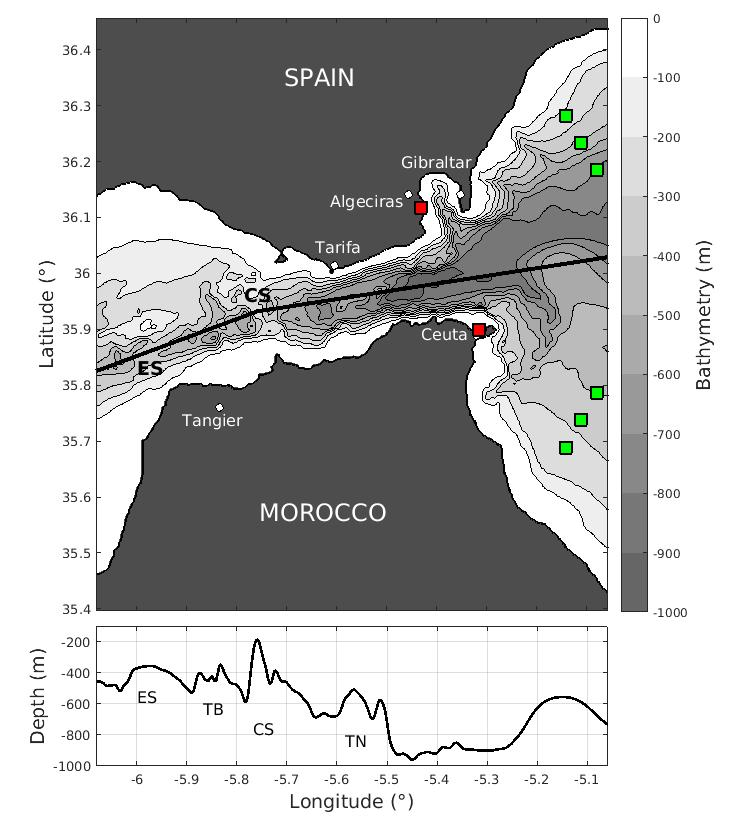
\includegraphics[width=5.66in,height=2.83in]{./media/image1.jpeg}
		\caption{ : Section verticale du champ de vitesse horizontale (doite-bas) et du champ d’anomalie de densité (droite-haut) à t=0.36T (T représente la période de M2) durant la phase de spin-up (initialisation « Lock-exchange ») dans 2D. (Panneaux de gauche) Profil vertical situé au-dessus de Camarinal Sill (localisé par les lignes rouge et bleue sur les panneaux de droite).}
		\label{fig:_Section_verticale_du_champ_de_vitesse_horizontale_doitebas_et_du_champ_danomalie_de_densit_droitehaut__t036T_T_reprsente_la_priode_de_M2_durant_la_phase_de_spinup_initialisation_Lockexchange_dans_2D_Panneaux_de_gauche_Profil_vertical_situ_audessus_de_Camarinal_Sill_localis_par_les_lignes_rouge_et_bleue_sur_les_panneaux_de_droite}
	\end{Center}
\end{figure}


%%%%%%%%%%%%%%%%%%%% Figure/Image No: 1 Ends here %%%%%%%%%%%%%%%%%%%%

\par

\begin{adjustwidth}{0.0in}{0.39in}
\par

\end{adjustwidth}

\begin{adjustwidth}{0.0in}{0.39in}
\begin{justify}
Nous avons évalué différents schémas numériques d’advection et de dissipation turbulente sur ces instabilités numériques. Dans la simulation numérique de référence, un schéma d’advection verticale « Splines» (respectivement « Akima ») avait initialement été utilisé pour la quantité de mouvement (respectivement pour les traceurs). 
\end{justify}\par

\end{adjustwidth}

\begin{adjustwidth}{0.0in}{0.4in}
\begin{justify}
Dans la simulation 2D, l’utilisation d’un schéma d’advection de type WENO d’ordre 5 sur la verticale pour les traceurs a permis de supprimer l’apparition d’instabilités numériques sur les champs de traceurs (cf Figure 3 – haut). Cependant, les instabilités numériques persistaient sur les champs de vitesse (cf Figure 3 – bas). Ce résultat a montré la nécessité pour la communauté CROCO de disposer de schémas d’advection verticale monotone (type TVD) ou quasi-monotone (type WENO) pour la quantité de mouvement (U, V en hydrostatique et W en version non-hydrostatique). 
\end{justify}\par

\end{adjustwidth}



%%%%%%%%%%%%%%%%%%%% Figure/Image No: 2 starts here %%%%%%%%%%%%%%%%%%%%

\begin{figure}[H]
	\begin{Center}
		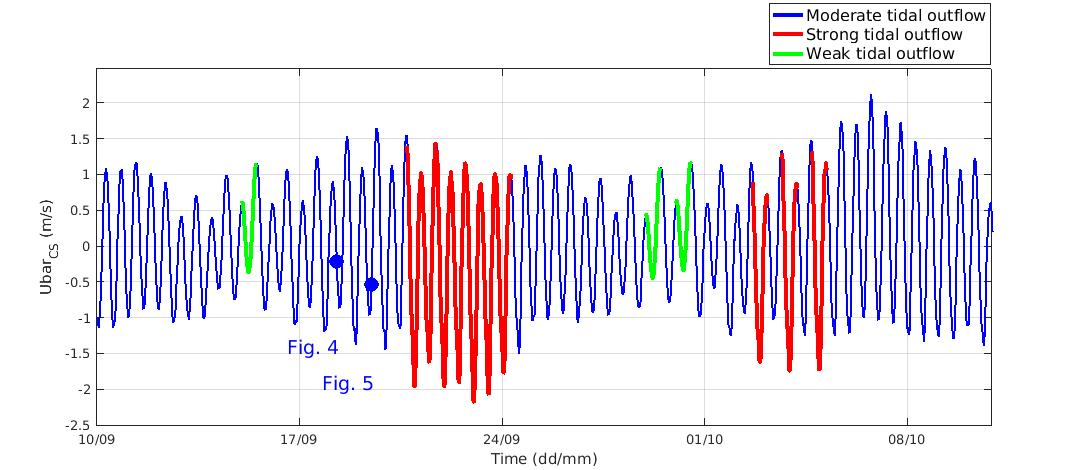
\includegraphics[width=4.98in,height=2.35in]{./media/image2.jpeg}
		\caption{ : Section verticale du champ de vitesse horizontale (doite-bas) et du champ d’anomalie de densité (droite-haut) à t=0.36T durant la phase de spin-up (initialisation « Lock-Exchange ») dans 2DTS-WENO5. (Panneaux de gauche) Profil vertical situé\  au-dessus de Camarinal Sill (localisé par les lignes rouge et bleue sur les panneaux de droite).}
		\label{fig:_Section_verticale_du_champ_de_vitesse_horizontale_doitebas_et_du_champ_danomalie_de_densit_droitehaut__t036T_durant_la_phase_de_spinup_initialisation_LockExchange_dans_2DTSWENO5_Panneaux_de_gauche_Profil_vertical_situ__audessus_de_Camarinal_Sill_localis_par_les_lignes_rouge_et_bleue_sur_les_panneaux_de_droite}
	\end{Center}
\end{figure}


%%%%%%%%%%%%%%%%%%%% Figure/Image No: 2 Ends here %%%%%%%%%%%%%%%%%%%%

\par

\begin{adjustwidth}{0.0in}{0.39in}
\par

\end{adjustwidth}

\begin{adjustwidth}{0.0in}{0.4in}
\begin{justify}
Des schémas d’advection TVD sont actuellement en cours de codage. La Figure 4 (bas) présente un premier résultat très encourageant avec la disparition des oscillations lorsqu’un tel schéma est utilisé pour l’advection verticale des composantes horizontales de la quantité de mouvement. 
\end{justify}\par

\end{adjustwidth}



%%%%%%%%%%%%%%%%%%%% Figure/Image No: 3 starts here %%%%%%%%%%%%%%%%%%%%

\begin{figure}[H]
	\begin{Center}
		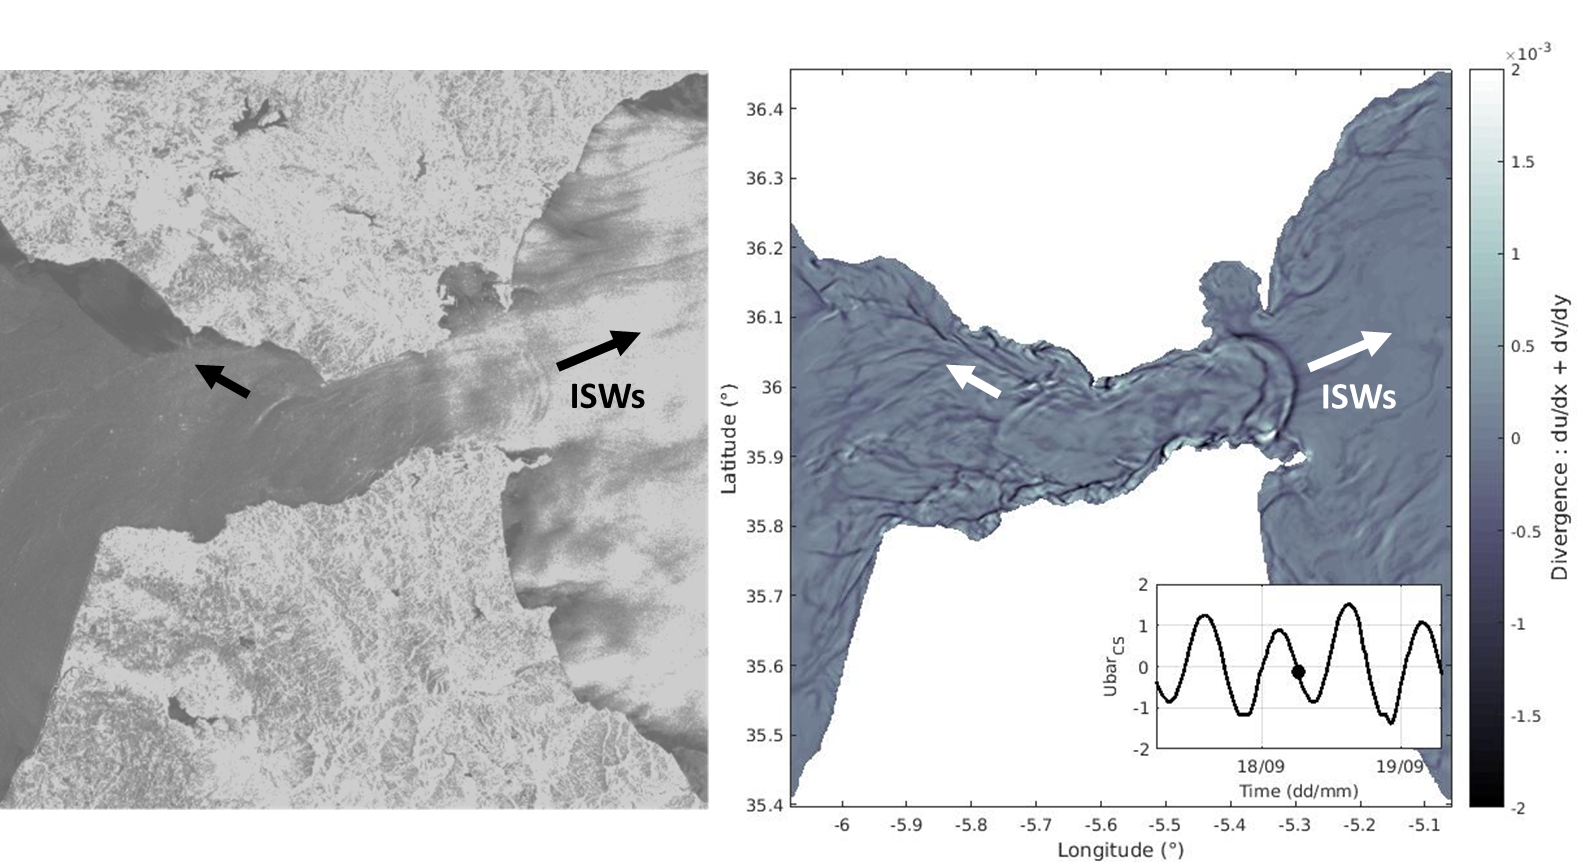
\includegraphics[width=5.68in,height=2.84in]{./media/image3.jpeg}
		\caption{: Section verticale du champ de vitesse horizontale (doite-bas) et du champ d’anomalie de densité (droite-haut) à t=0.36T durant la phase de spin-up (initialisation « Lock-exchange ») dans 2DTS-WENO5,UV-TVD. (Panneaux de gauche) Profil vertical situé au dessus de Camarinal Sill (localisé par les lignes rouge et bleue sur les panneaux de droite).}
		\label{fig:_Section_verticale_du_champ_de_vitesse_horizontale_doitebas_et_du_champ_danomalie_de_densit_droitehaut__t036T_durant_la_phase_de_spinup_initialisation_Lockexchange_dans_2DTSWENO5UVTVD_Panneaux_de_gauche_Profil_vertical_situ_au_dessus_de_Camarinal_Sill_localis_par_les_lignes_rouge_et_bleue_sur_les_panneaux_de_droite}
	\end{Center}
\end{figure}


%%%%%%%%%%%%%%%%%%%% Figure/Image No: 3 Ends here %%%%%%%%%%%%%%%%%%%%

\par

\begin{adjustwidth}{0.0in}{0.39in}
\par

\end{adjustwidth}

\begin{adjustwidth}{0.0in}{0.4in}
\begin{justify}
Les premiers résultats, très encourageants, obtenus avec les schémas d’advection de type TVD et WENO confirment, si besoin est, un certain nombre de choix numériques assez fondamentaux de la communauté CROCO concernant l’utilisation de schémas numériques « monotones » ou « quasi-monotones ». Les tests de sensibilité réalisés dans le cadre de la présente étude ont toutefois montré qu’il était possible de supprimer les oscillations numériques obtenus avec des schémas numériques non monotones plus classiques mais en ayant recours à une dissipation numérique jugée trop importante (coefficient de mélange vertical > 0.001 m²/s $\&$  coefficient de viscosité $ \geq $  0.1 m²/s) et en tout cas incompatible avec la simulation des trains de solitons observés en aval du détroit (dissipation numérique des trains d’ondes : sous-estimation de l’amplitude des solitons et de leur zone de propagation) . Nous avons donc choisi de ne pas poursuivre l’implémentation ou l’évaluation de techniques plus sophistiquées pour la modélisation des processus sous-maille et la modélisation des fronts, nous orientant vers des schémas numériques monotones d’advection jugés plus « physiques » et offrant de meilleurs résultats numériques. Les maquettes CROCO (hydrostatiques et non-hydrostatiques) à très haute résolution mises en place dans le cadre du présent contrat nous permettront de tester dans un très proche avenir les premières simulations numériques de type ILES (\textit{pour Implicit Large Eddy Simulation) }voire MILES \textit{(pour Monotone Implicit Large Eddy Simulation).}
\end{justify}\par

\end{adjustwidth}


\vspace{\baselineskip}
\begin{justify}
Suite à l’observation dans la simulation 2DV, d’oscillations numériques dans les zones de forts cisaillements de vitesse, des schémas d’advection TVD pour l’advection verticale et horizontale des composantes horizontales (U-V) et verticale (W) de la quantité de mouvement ont été développé dans le modèle CROCO. Ces schémas ont été codés avec différentes options de limiteurs plus ou moins diffusifs (MINMOD, VanLeer, SUPERBEE). Nous avons évalué l’impact de ces nouveaux schémas numériques d’advection sur les champs de vitesse horizontale de la simulation 3D NH-REF. La Figure 3 : présente des résultats très encourageants : l’utilisation de ces schémas permet de supprimer totalement l’apparition d’instabilités numériques sur les champs de vitesses horizontales U au-dessus des reliefs abruptes (figure du milieu et du bas).
\end{justify}\par


\vspace{\baselineskip}


%%%%%%%%%%%%%%%%%%%% Figure/Image No: 4 starts here %%%%%%%%%%%%%%%%%%%%

\begin{figure}[H]
	\begin{Center}
		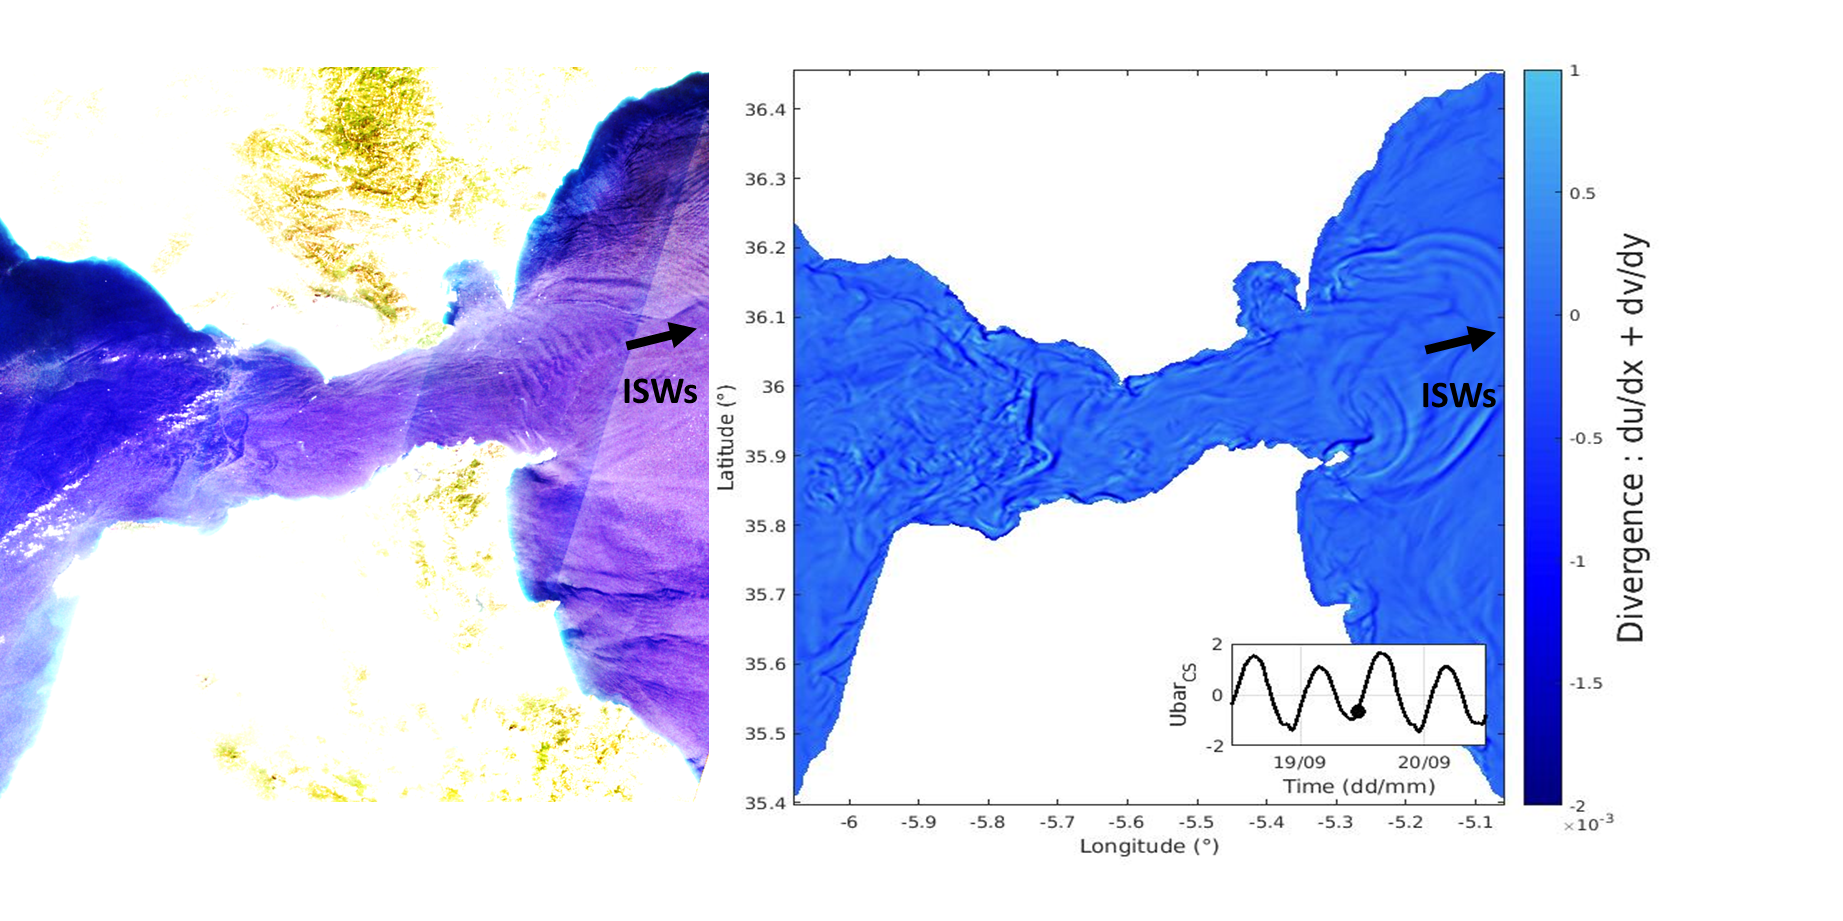
\includegraphics[width=6.29in,height=3.55in]{./media/image4.png}
		\caption{ : Test de sensibilité du champ de vitesse horizontale aux schémas d’advection de la quantité de mouvement. (haut) Section verticale du champ de vitesse horizontale à t=1.36T dans la maquette 3DUP3-SPLINES. (milieu) Section verticale du champ de vitesse horizontale à t=1.36T dans la maquette 3DTVD-SUPERBEE. (bas) Section verticale du champ de vitesse horizontale à t=1.36T dans la maquette 3DTVD-MINMOD.}
		\label{fig:_Test_de_sensibilit_du_champ_de_vitesse_horizontale_aux_schmas_dadvection_de_la_quantit_de_mouvement_haut_Section_verticale_du_champ_de_vitesse_horizontale__t136T_dans_la_maquette_3DUP3SPLINES_milieu_Section_verticale_du_champ_de_vitesse_horizontale__t136T_dans_la_maquette_3DTVDSUPERBEE_bas_Section_verticale_du_champ_de_vitesse_horizontale__t136T_dans_la_maquette_3DTVDMINMOD}
	\end{Center}
\end{figure}


%%%%%%%%%%%%%%%%%%%% Figure/Image No: 4 Ends here %%%%%%%%%%%%%%%%%%%%

\par

\par

\begin{justify}
Nous avons également évalué l’impact de ces nouveaux schémas numériques sur la propagation des trains d’ondes solitaires dans la simulation 3D-NH REF : sur la Figure 4, on observe que les schémas d’advection de type TVD (MINMOD, VanLeer $\&$  SUPERBEE) ont tendance à dissiper un peu plus les ondes solitaires que les schémas d’advection UP3 et SPLINES (amplitude et vitesse verticale associé aux solitons plus faibles). Cependant, l’utilisation du limiteur SUPERBEE permet de réduire significativement ces effets dissipatifs. Une nouvelle version des schémas d’advection TVD moins dissipative est actuellement en développement.
\end{justify}\par



%%%%%%%%%%%%%%%%%%%% Figure/Image No: 5 starts here %%%%%%%%%%%%%%%%%%%%

\begin{figure}[H]
	\begin{Center}
		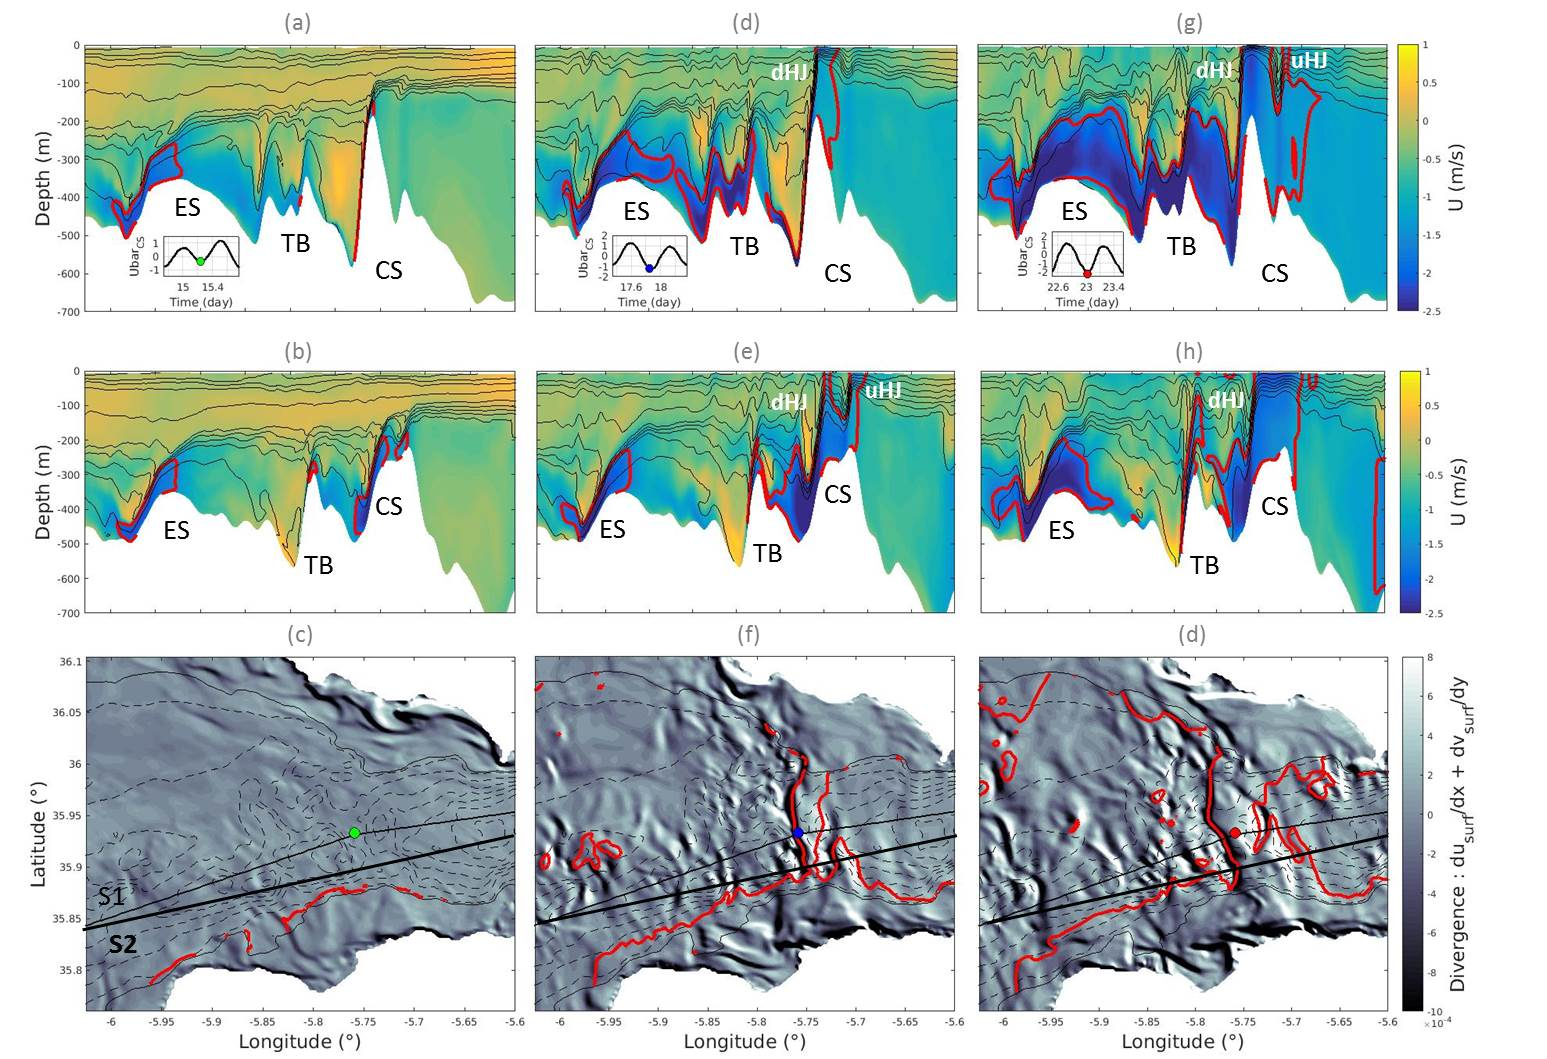
\includegraphics[width=6.3in,height=2.91in]{./media/image5.png}
		\caption{: Test de sensibilité des trains d’ondes solitaires aux schémas d’advection de la quantité de mouvement.\ \ \ \ \ \   Sections verticales des champs d’anomalie de densité et de vitesse verticale à t=1.1T : (a)  pour la maquette 3DTVD-MINMOD, (b) pour la maquette 3DTVD-VanLeer,\  (c)  pour la maquette 3DTVD-SUPERBEE, (d) pour la maquette 3DUP3-SPLINES.}
		\label{fig:_Test_de_sensibilit_des_trains_dondes_solitaires_aux_schmas_dadvection_de_la_quantit_de_mouvement________Sections_verticales_des_champs_danomalie_de_densit_et_de_vitesse_verticale__t11T_a__pour_la_maquette_3DTVDMINMOD_b_pour_la_maquette_3DTVDVanLeer__c__pour_la_maquette_3DTVDSUPERBEE_d_pour_la_maquette_3DUP3SPLINES}
	\end{Center}
\end{figure}


%%%%%%%%%%%%%%%%%%%% Figure/Image No: 5 Ends here %%%%%%%%%%%%%%%%%%%%

\par

\par


\vspace{\baselineskip}

\vspace{\baselineskip}

\printbibliography
\end{document}